\documentclass[12pt]{article}
\usepackage[utf8]{inputenc}
\usepackage{graphicx} % For including images
\usepackage{geometry} % For page size and margins
\geometry{a4paper, margin=0.8in}

\title{Hospital Management System}
\author{Muhammad Rehan \\ 22P-9106}
\date{Assignment 03}
\begin{document}

\maketitle

\section*{Assignment Abstract}
In this assignment of the project, I am advancing the Hospital Management System by defining and finalizing the design model, which is a crucial step before writing the actual code. This process involves identifying relevant classes and objects based on previously gathered requirements and user stories, and establishing associations between them. The output will be a comprehensive class diagram that includes all attributes, functions, and associations, with sequence diagrams that tell the interactions and workflows between objects. This assignment aims to ensure that our design is fully aligned with the analysis models developed in assignment one, resulting in preparing a robust foundation for the coding phase.

\section*{Identification of Classes and Objects}
\subsection*{Overview}
To make the foundation of our design model, I begin by identifying potential classes and objects from the case study. These classes represent the primary entities of our system, each encapsulating essential data and functions relevant to the operations of the hospital management system.

\subsection*{Classes and Objects}
There is the detailed list of identified classes along with a brief description of their roles within the system, reflecting the implementation details in the class diagram:

\begin{itemize}
  \item \textbf{Person (Abstract)}: A base class for all individuals involved in the system, providing common attributes like name, address, and phone, and a method to update profiles.
  \item \textbf{Patient}: Inherits from Person; represents individuals receiving care, capable of registering, logging in, and managing appointments. They hold unique identifiers and personal information.
  \item \textbf{Employee (Abstract)}: Inherits from Person; a base class for all employees, including doctors, nurses, and administrative staff, incorporating common employee attributes such as employeeID.
  \item \textbf{Doctor}: Inherits from Employee; healthcare providers who diagnose, treat, and manage patient care, capable of prescribing medications.
  \item \textbf{Nurse}: Inherits from Employee; responsible for patient assessments and supporting doctors in preliminary care.
  \item \textbf{Admin Staff}: Inherits from Employee; includes roles such as Receptionists who manage operational and administrative tasks.
  \item \textbf{Appointment}: A scheduled medical or administrative service provided to a patient, implementing the Billable interface for charging purposes.
  \item \textbf{Medical Record}: Compositionally linked to Patients; contains comprehensive data about patient diagnoses, treatments, and health history.
  \item \textbf{Prescription}: Issued by doctors, detailing medications for patients.
  \item \textbf{Bill}: Implements the Billable interface; financial documentation for services provided, linked to patients and payments.
  \item \textbf{LabTest}: Implements the Billable interface; represents tests ordered by doctors, including costs and results processing.
  \item \textbf{Pharmacy}: Manages and dispenses prescribed medications, maintaining stock and medication details.
\end{itemize}

\section*{Identification of Associations}
\subsection*{Overview}
With the classes clearly defined, I now proceed to delineate the relationships and interactions among them. These associations are important for understanding how objects coexist and collaborate within the system.

\subsection*{Associations}
\begin{itemize}
  \item \textbf{Patient to Doctor}: Many-to-many relationship facilitated through Appointments, indicating that patients can consult multiple doctors and vice versa.
  \item \textbf{Doctor to Prescription}: One-to-many relationship, where a doctor can issue multiple prescriptions to various patients.
  \item \textbf{Patient to Medical Record}: One-to-one relationship, signifying that each patient has a unique medical record.
  \item \textbf{Appointment to Receptionist}: Many-to-one relationship, where multiple appointments are managed by a receptionist, reflecting their role in scheduling and administrative tasks.
  \item \textbf{LabTest to Doctor and Patient}: Many-to-many relationship, where multiple lab tests can be ordered by various doctors for different patients, showing the interconnectivity between diagnostic procedures and patient care.
\end{itemize}

\begin{figure}[h!]
\centering
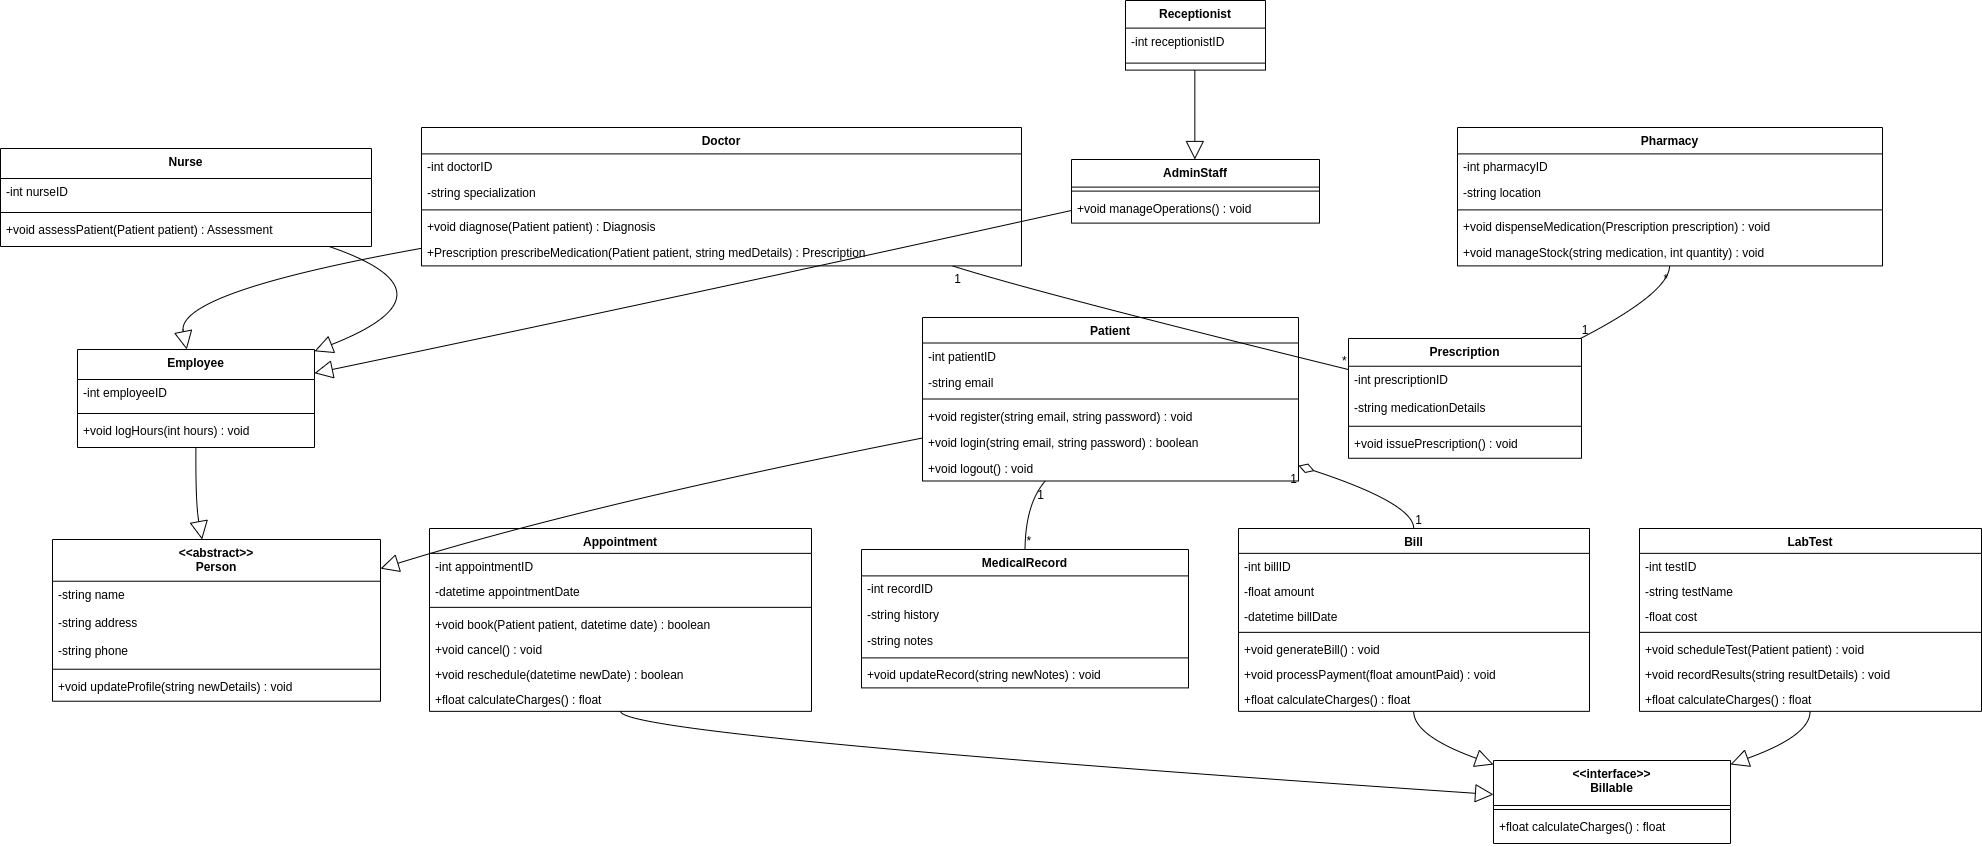
\includegraphics[width=1\textwidth]{1.png}
\caption{Class Diagram}
\end{figure}


\section*{Sequence Diagrams}
Now comes the second part of the assignment which has detailed descriptions of sequence diagrams for key use cases within the Hospital Management System. 

\subsection*{Patient Registration}
The Patient Registration sequence diagram shows the steps involved when a new patient registers in the system. The process begins with the patient accessing the registration page, entering their details, and submitting them. The system validates and processes these details, creating a new patient record in the database, and confirming successful registration to the patient.

\begin{figure}[h!]
\centering
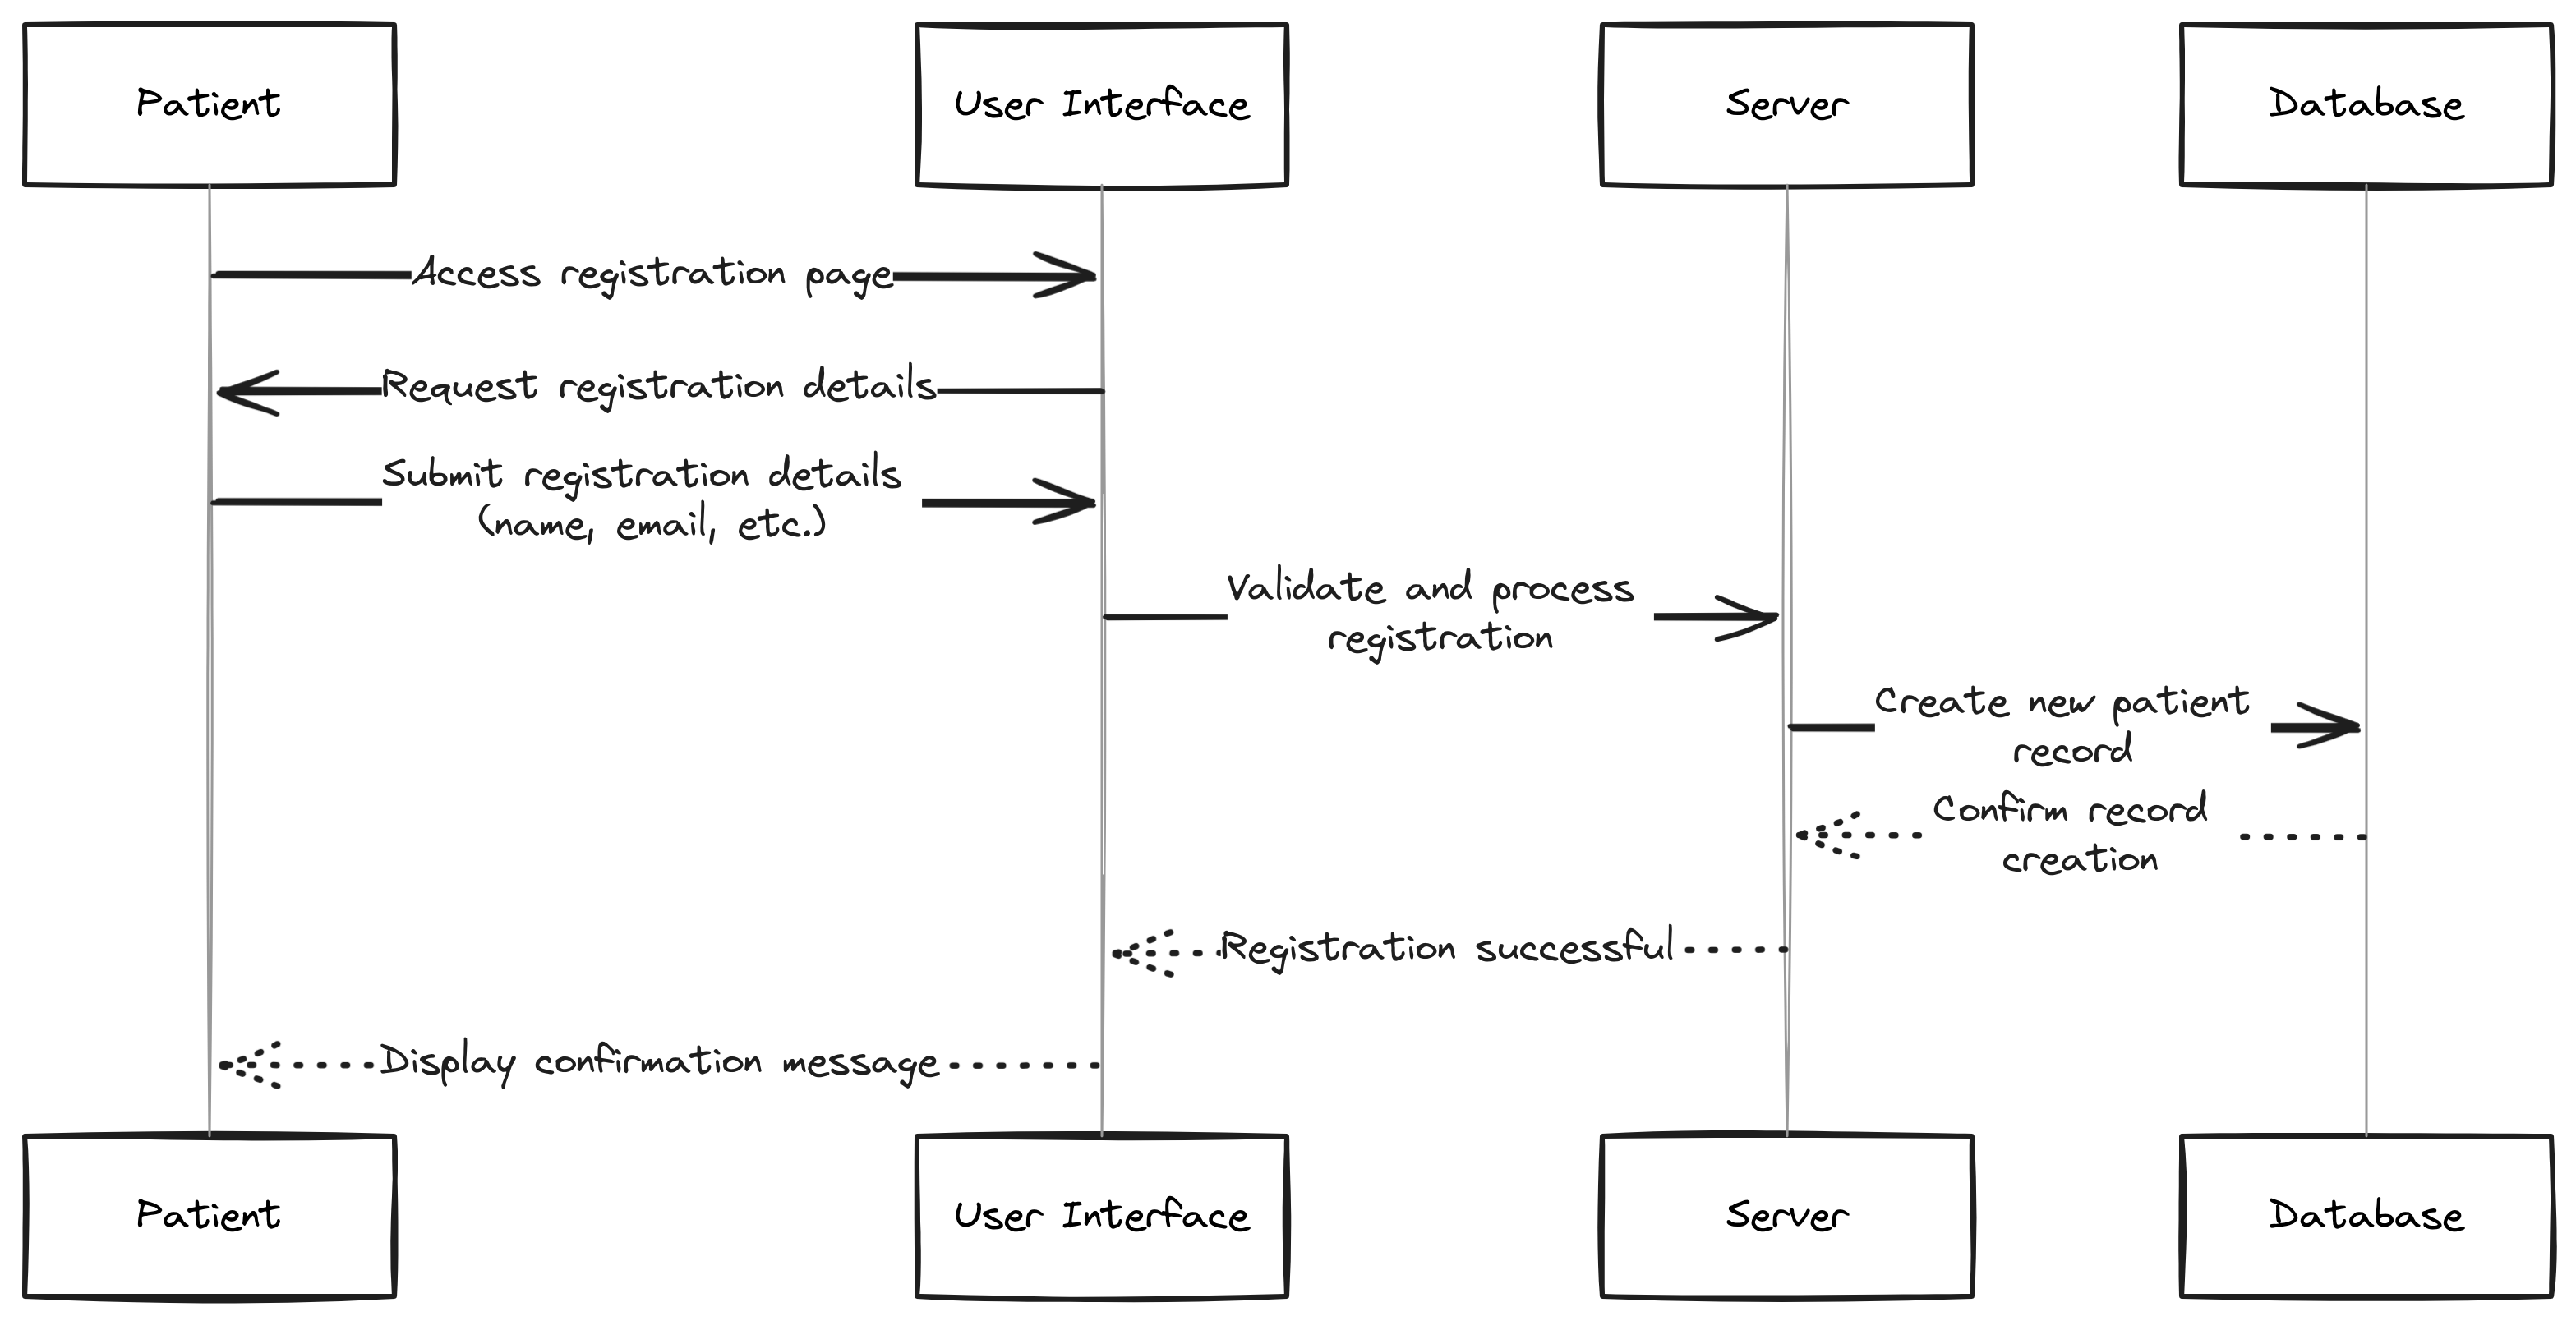
\includegraphics[width=0.8\textwidth]{patient_registration_diagram.png}
\caption{Sequence diagram for Patient Registration}
\end{figure}

\subsection*{Booking an Appointment}
The Booking an Appointment sequence shows depicts the interactions required for a patient to book an appointment. The patient logs into the system, requests an appointment, and selects a preferred time and doctor based on availability. The system communicates with the receptionist to confirm and schedule the appointment, updating the database accordingly and notifying the patient of the successful booking.

\begin{figure}[h!]
\centering
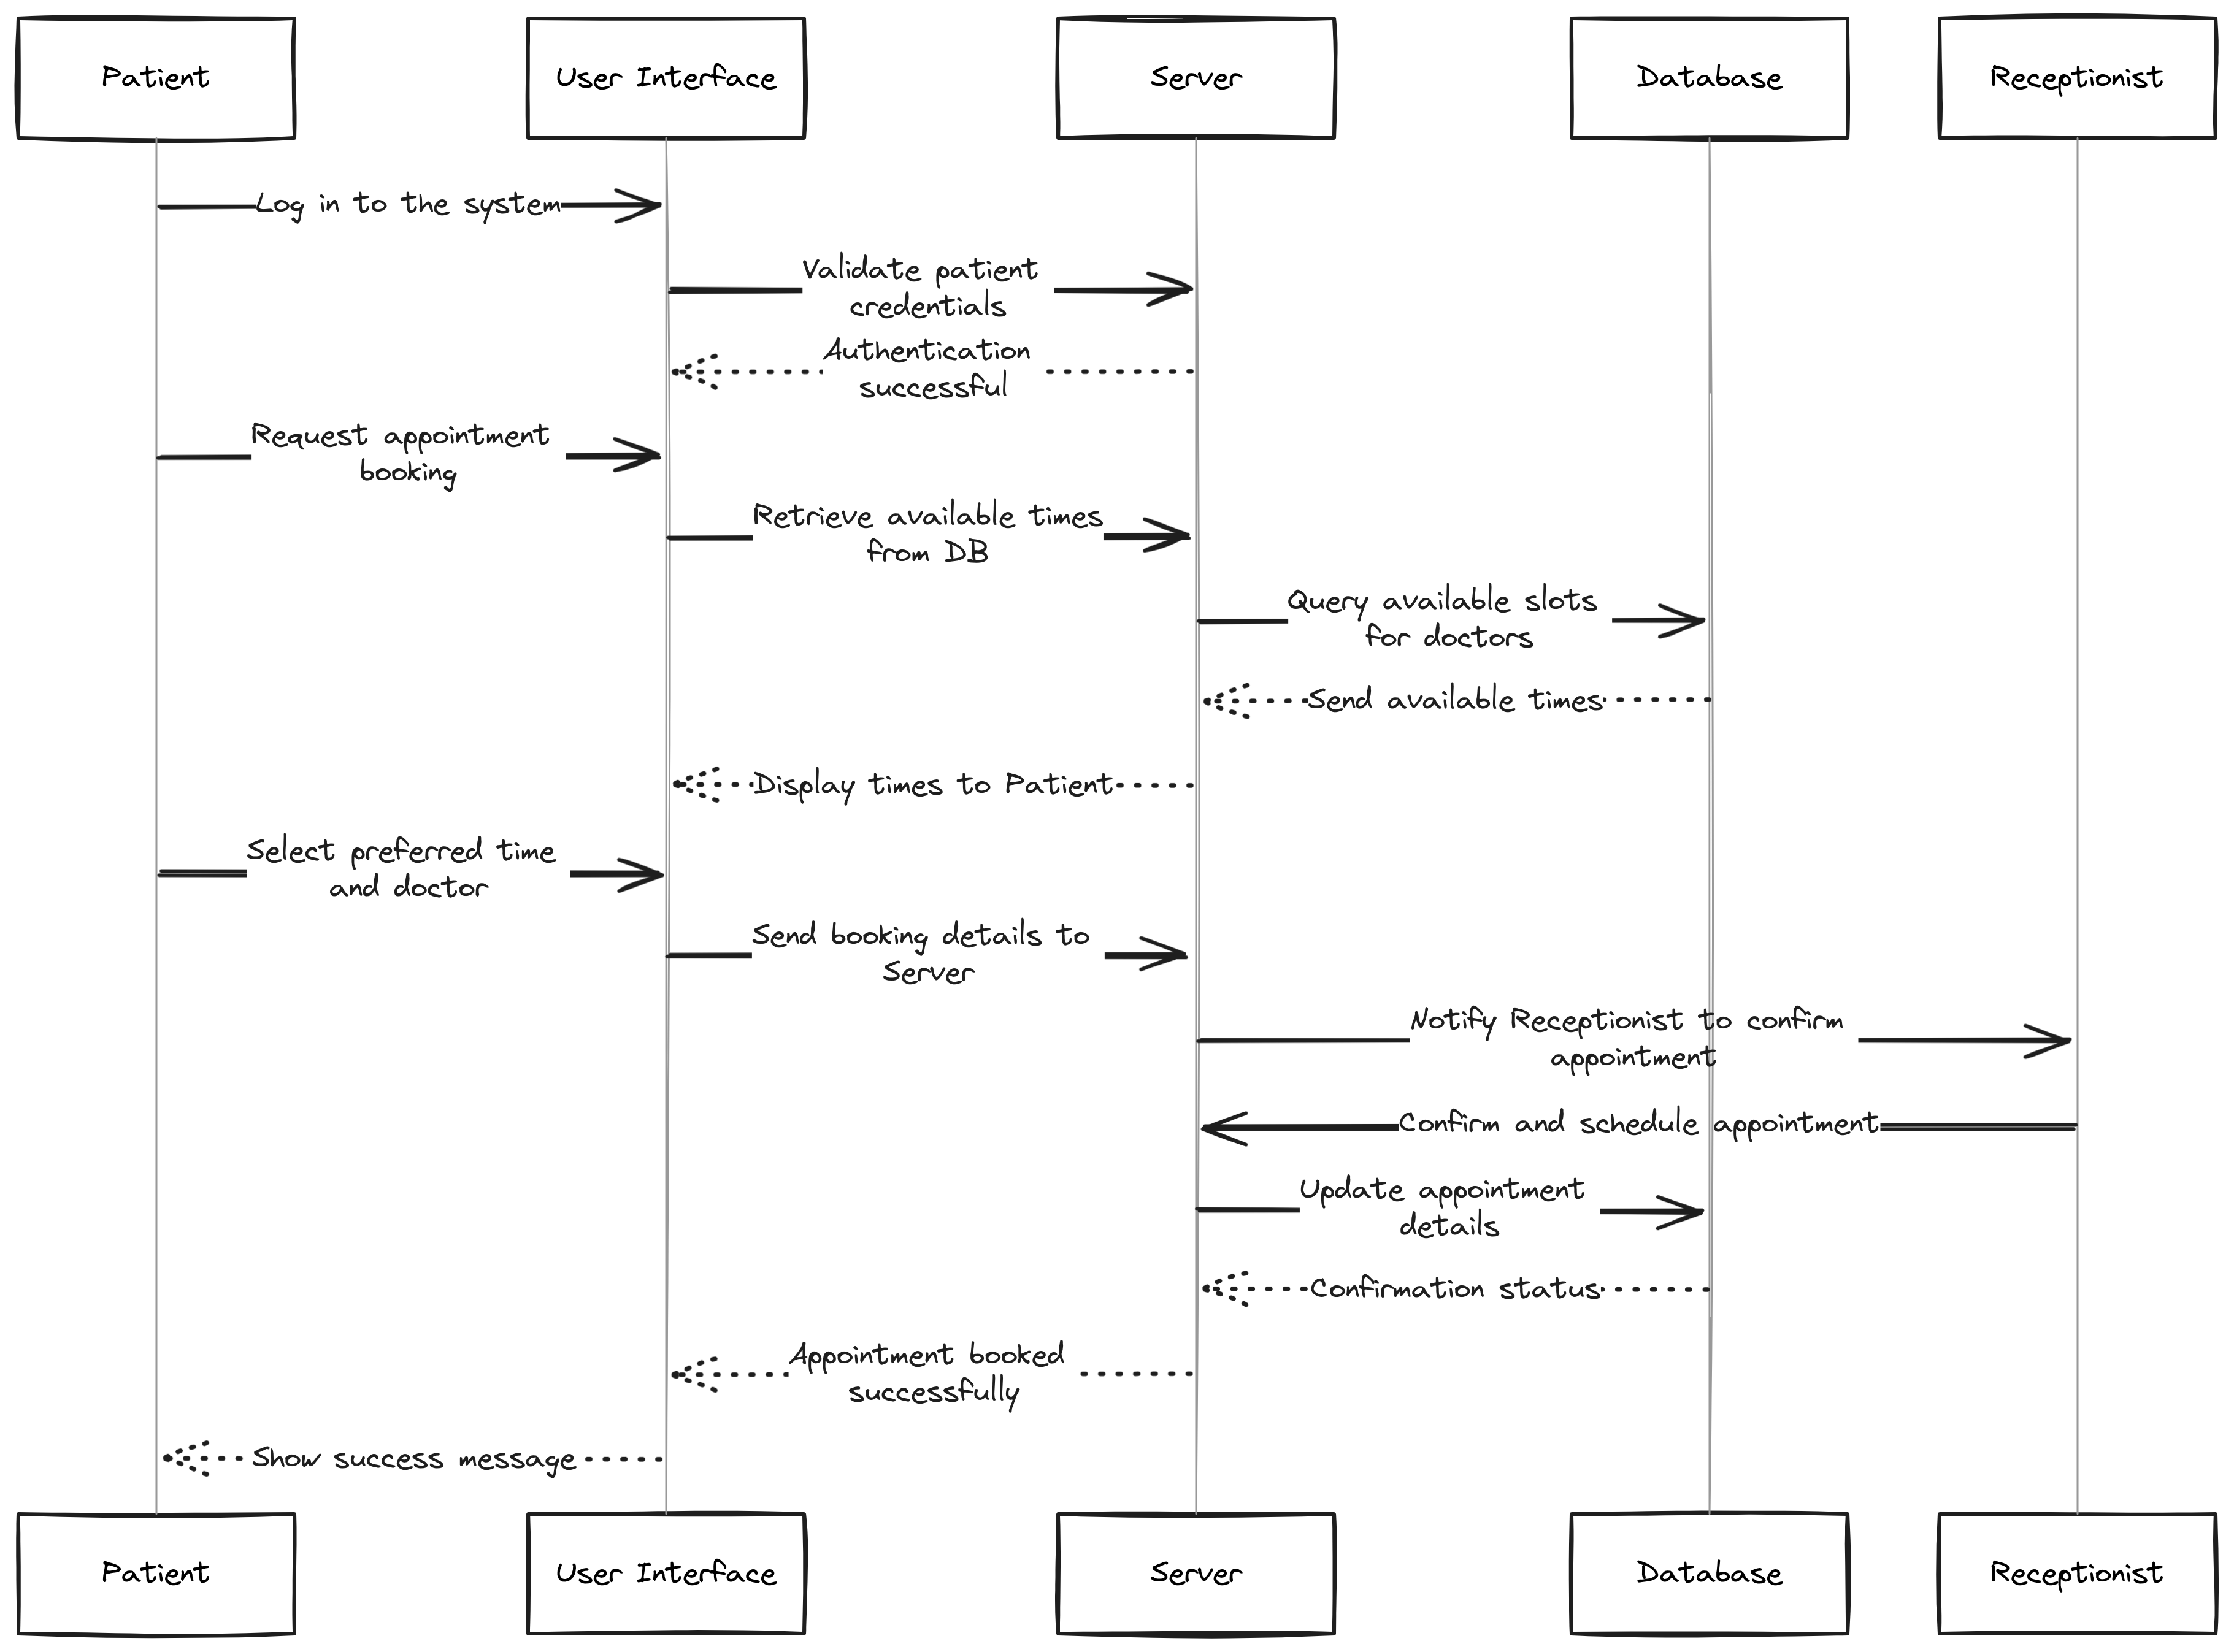
\includegraphics[width=0.8\textwidth]{booking_appointment_diagram.png}
\caption{Sequence diagram for Booking an Appointment}
\end{figure}

\subsection*{Medical Consultation}
The Medical Consultation sequence diagram shows the sequence of interactions during a doctor's consultation with a patient. This includes the nurse's initial assessment, the doctor reviewing the patient's medical history, updating the medical record with new information, and concluding with the doctor providing a diagnosis and treatment plan.

\begin{figure}[h!]
\centering
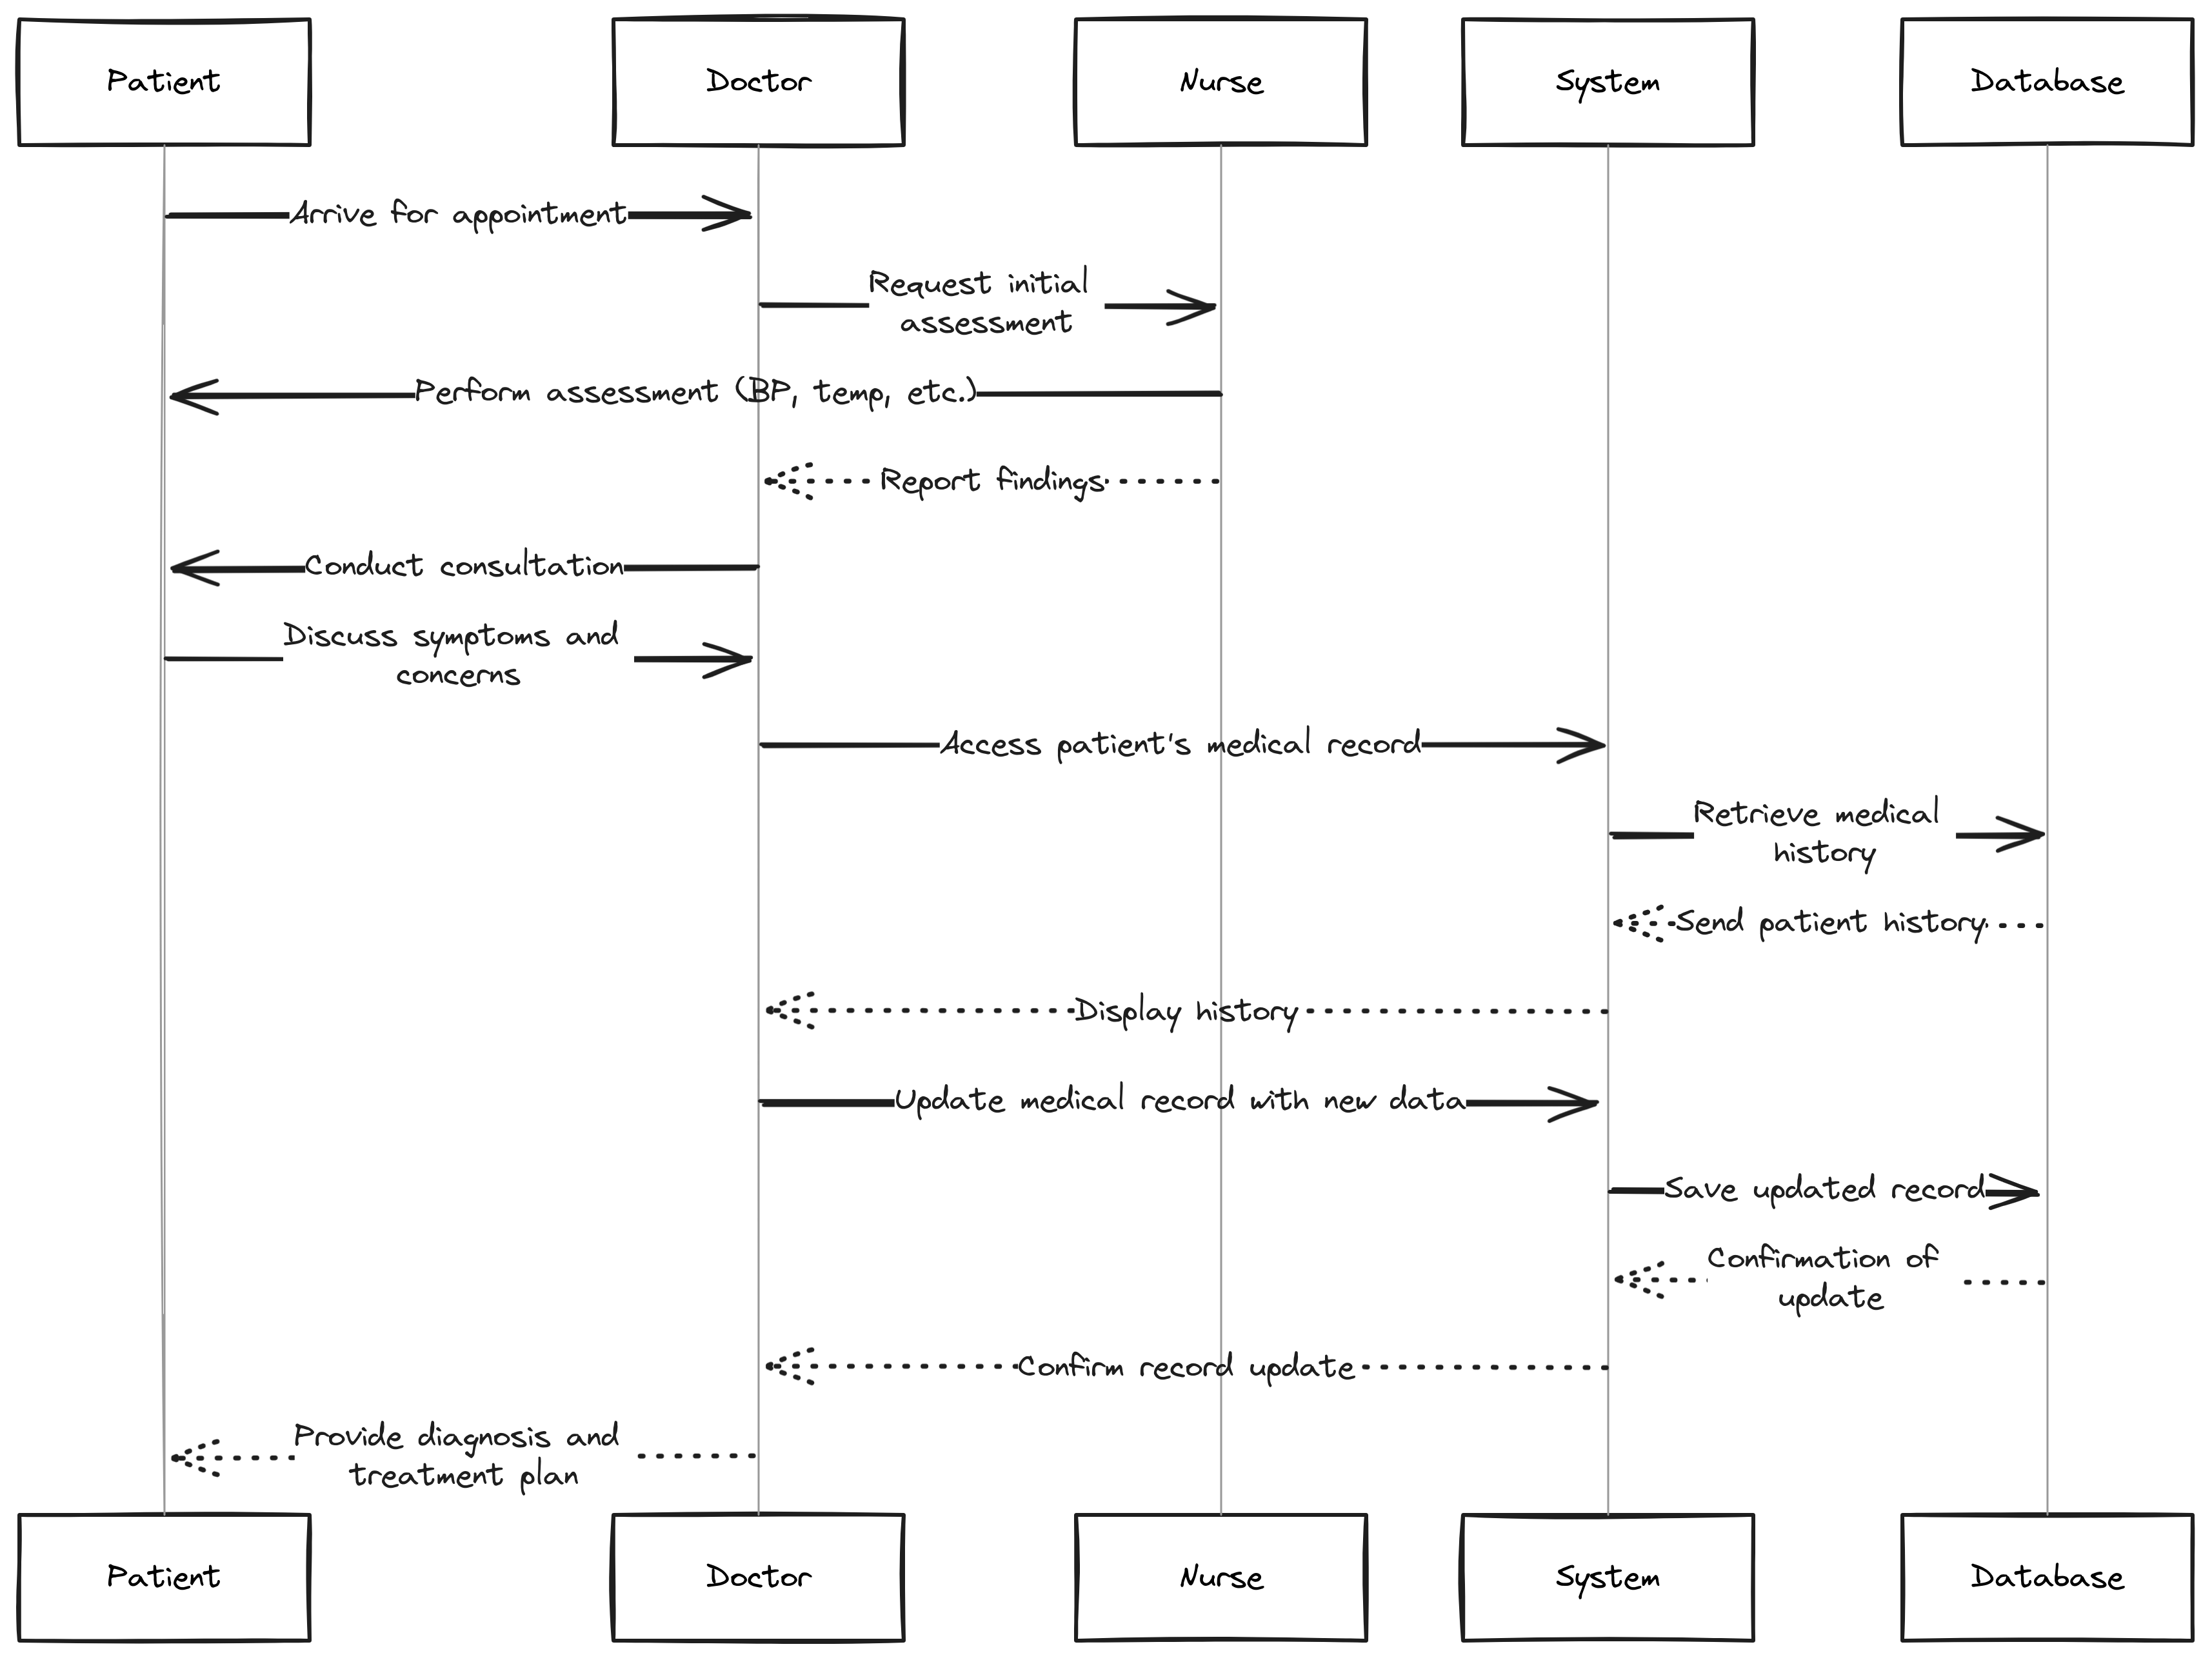
\includegraphics[width=0.8\textwidth]{medical_consultation_diagram.png}
\caption{Sequence diagram for Medical Consultation}
\end{figure}

\newpage


\subsection*{Prescription and Pharmacy Interaction}
The Prescription and Pharmacy Interaction sequence diagram shows how a prescription is created by the doctor, stored in the system, and then retrieved and fulfilled by the pharmacy. This process involves multiple system validations and updates, ensuring the prescription details are accurately handled and the medications are correctly dispensed to the patient.

\begin{figure}[h!]
\centering
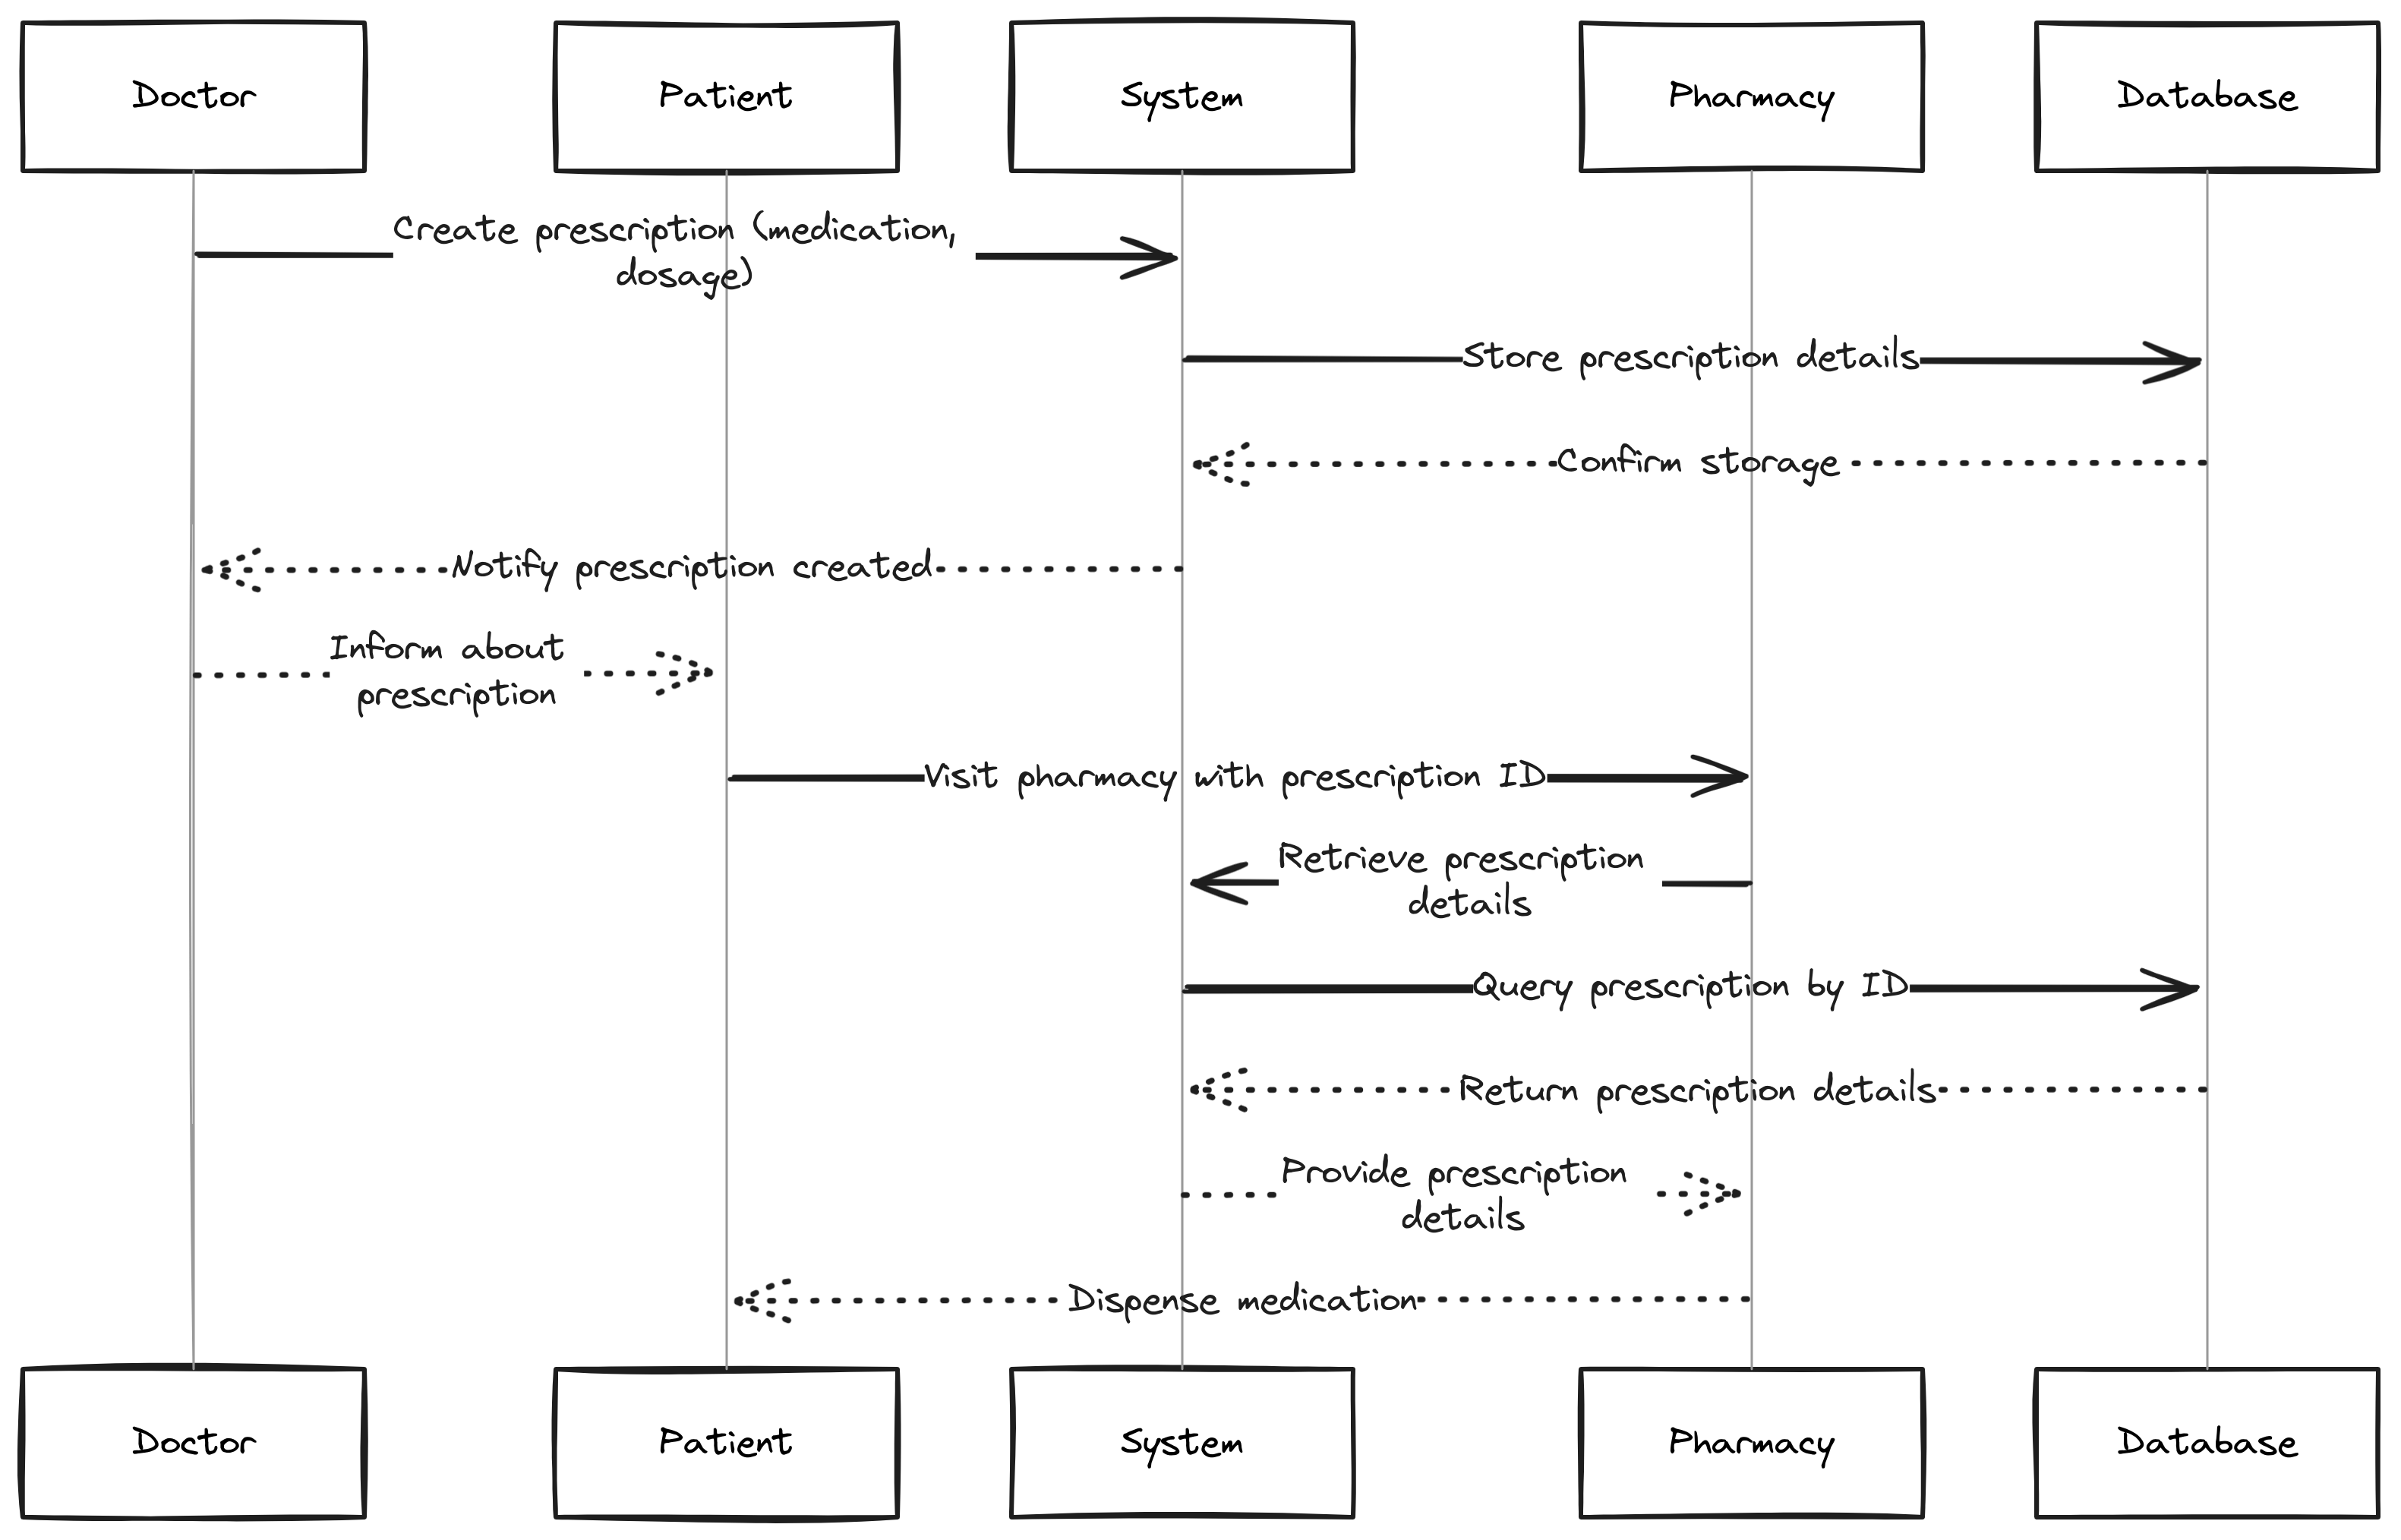
\includegraphics[width=0.8\textwidth]{prescription_pharmacy_interaction_diagram.png}
\caption{Sequence diagram for Prescription and Pharmacy Interaction}
\end{figure}

These diagrams are important for visualizing the dynamic aspects of the system's operations, providing a clear guide for development and implementation phases.

\noindent\hrulefill


\end{document}
